\documentclass[12pt,a4paper]{article}
\usepackage[utf8]{inputenc}
\usepackage[english]{babel}
\usepackage[T1]{fontenc}
\usepackage{amsmath}
\usepackage{amsfonts}
\usepackage{amssymb}
\usepackage{graphicx}
\usepackage{siunitx}
\usepackage{float}
\usepackage[left=2cm,right=2cm,top=2cm,bottom=2cm]{geometry}
\author{Gerald}

\begin{document}
\sisetup{separate-uncertainty = true}
	\setlength{\parindent}{0pt} 
	\begin{center}
		{\LARGE Experiment protocol}\\
		\begin{large}
			for the solid state lab course\\[0.4cm]
			at RWTH Aachen\\
			II. Physikalisches Institut A\\[5.5cm]
			\Large\textbf{\textsl{Raman characterization of CVD grown graphene and 2D material based heterostructures}}\\[5.5cm]
			\normalsize\textit{authored\\by}\\[0.4cm]
			\large{Moritz Berger (355244)\\Gerald Kolter (355005)}\\[2cm]
			\large \textbf{Summer term 2019}
		\end{large}
	\end{center}
	\newpage
	
	\tableofcontents
	\newpage

\section{Introduction}








%\begin{figure} [H]
%\centering
%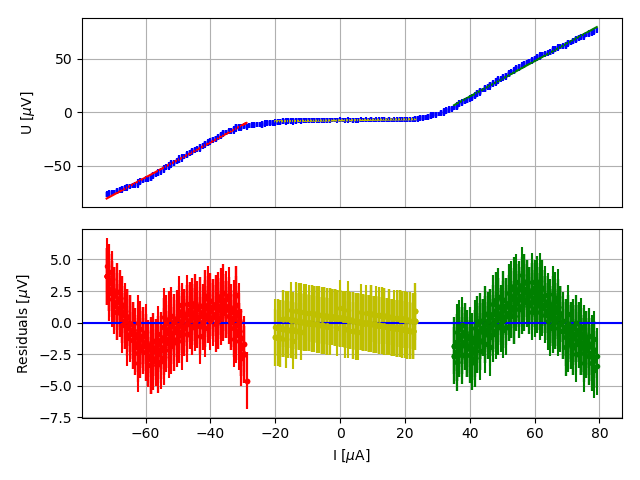
\includegraphics[scale=0.8]{Bilder/U_I_characteristic/fit_43.PNG}
%\caption{U-I characteristic of the SQUID in the superconducting state.}
%\label{fig:U-I-characteristic_fit}
%\end{figure}

%\begin{table} [H]
%\centering
%\begin{tabular}{|c|c|c|c|}
%\hline 
%$T_{room}$ [K] & $T_{LN_2}$ [K] & $R_{RT}$ [k$\Omega$] & $R_{LN_2}$ [k$\Omega$] \\ 
%\hline 
%294.65 $\pm$ $\frac{1}{\sqrt{12}}$ & 77 $\pm$ $\frac{1}{\sqrt{12}}$ & 107.9 $\pm$ $\frac{1}{\sqrt{12}}$ & 20.3 $\pm$ $\frac{1}{\sqrt{12}}$ \\ 
%\hline 
%\end{tabular} 
%\caption{Measured values for the resistance at room temperature and the temperature of liquid nitrogen.}
%\label{tab:Temp_Calib_data}
%\end{table}




\end{document}